\documentclass[a4paper, 12pt]{article}

\usepackage{hyperref}
\usepackage[warn]{mathtext}
\usepackage[utf8]{inputenc}
\usepackage[T2A]{fontenc}
\usepackage[english,russian]{babel}
\usepackage{multirow}
\usepackage{float}
\restylefloat{table}
\usepackage{amsmath,amsfonts,amssymb,amsthm,mathtools}
\usepackage{indentfirst}
\DeclareSymbolFont{T2Aletters}{T2A}{cmr}{m}{it}
\usepackage{ gensymb }
\mathtoolsset{showonlyrefs=true}
\usepackage{euscript}
\usepackage{mathrsfs}
\usepackage[left=2cm,right=2cm,top=2cm,bottom=2cm]{geometry}
\usepackage{graphicx}
\usepackage{wrapfig}
\usepackage[rgb]{xcolor}
\hypersetup{
colorlinks=true,
urlcolor=blue
}
\usepackage{tikz}

\title{Лабораторная работа}
\author{Гисич Арсений Б03-102}
\date{2023}

\begin{document}

	\begin{center}
		{\large МОСКОВСКИЙ ФИЗИКО-ТЕХНИЧЕСКИЙ ИНСТИТУТ (НАЦИОНАЛЬНЫЙ ИССЛЕДОВАТЕЛЬСКИЙ УНИВЕРСИТЕТ)}
	\end{center}
	\vspace{5 cm}
	{\Large
		\begin{center}
			{\bf Лабораторная работа 4.7.3}\\[0.2 cm]
			Поляризация
		\end{center}
	}
	\vspace{4 cm}
	\begin{flushright}
		{\Large Выполнили: \\
			\vspace{0.2 cm}
			Гисич Арсений \\
            Айрапетян Микаел \\
			\vspace{0.2 cm}
			Б03-102 \\}
	\end{flushright}
	\vspace{8 cm}
	\begin{center}
		Долгопрудный\\[0.1 cm]
		2023
	\end{center}
\thispagestyle{empty}

\section{Аннотация}

В данной работе при помощи чёрного зеркала были определены разрешённые направления поляроидов; был определён характер поляризации света, прошедшего стопу и отражённого от неё под углом Брюстера; был оценён угол Брюстера для эбонита; были выделены пластинки $\lambda/2$ и $\lambda/4$; определены направления большей и меньшей скоростей для пластинки $\lambda/4$; была исследована интерференция поляризованных лучей.

\section{Теоретические сведения}

\subsection{Определение направления разрешённой плоскости колебаний поляроида}
	
	Определить направление разрешённых колебаний поляроида проще всего с помощью чёрного зеркала.
	
При падении света на отражающую поверхность под углом Брюстера, свет в отражённом луче почти полностью поляризован, а вектор E
параллелен отражающей поверхности ("<правило иголки">). Луч света,
прошедший поляроид и отразившийся от чёрного зеркала, имеет минимальную интенсивность при выполнении двух условий: во-первых, свет
падает на отражающую поверхность под углом Брюстера и, во-вторых,
в падающем пучке вектор E лежит в плоскости падения.

Вращая поляроид вокруг направления луча и чёрное зеркало вокруг
оси, перпендикулярной лучу, методом последовательных приближений
можно добиться минимальной яркости луча, отражённого от зеркала,
и таким образом определить разрешённое направление поляроида.

Измеряя угол поворота зеркала (угол Брюстера), нетрудно определить коэффициент преломления материала, из которого изготовлено
зеркало. Описанный метод часто используется для измерения коэффициента преломления непрозрачных диэлектриков.

\subsection{Получение эллиптически поляризованного света}
\begin{wrapfigure}{r}{0.35\linewidth} 
	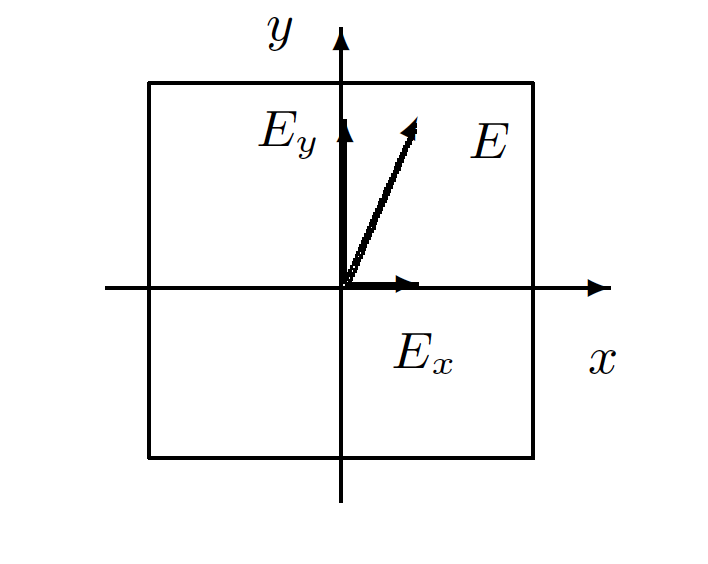
\includegraphics[width=\linewidth]{1.png}
	\caption{Разложение линейно поляризованного света по главным направлениям двоякопреломляющей пластинки}
	\label{ris 1}
\end{wrapfigure}

Эллиптически поляризованный свет можно получить из линейно поляризованного с
помощью двоякопреломляющих кристаллических пластинок.

Двоякопреломляющая пластинка имеет два взаимно перпендикулярных главных направления, совпадающих с осями эллипсоида диэлектрической проницаемости. Волны, поляризованные вдоль главных направлений, распространяются в пластинке с разными скоростями, не изменяя характера своей поляризации. Эти волны называются главными. Мы будем обозначать показатели преломления для главных волн через $ n_x $ и $ n_y $, где $ x $ и $ y $ --- главные направления кристаллической пластинки (рис. 1).

Пусть на пластинку падает линейно поляризованная волна, электрический вектор которой ориентирован под некоторым углом $ \alpha $ к оси
$ x $. Разложим вектор $ \mathbf{E} $ на составляющие $ E_x $ и $ E_y $. На входе пластинки $ E_x $ и $ E_y $ находятся в фазе. На выходе из-за разности скоростей между ними появляется разность хода $ d(n_x - n_y) $, при этом сдвиг фаз определяется соотношением

\begin{equation}\label{}
\Delta \phi =  \dfrac{2\pi}{m} = k d(n_x - n_y)
\end{equation}
Как уже отмечалось, при сложении двух взаимно перпендикулярных колебаний, обладающих некоторым сдвигом фаз, образуется колебание, поляризованное по эллипсу.

\begin{wrapfigure}{l}{0.35\linewidth}
	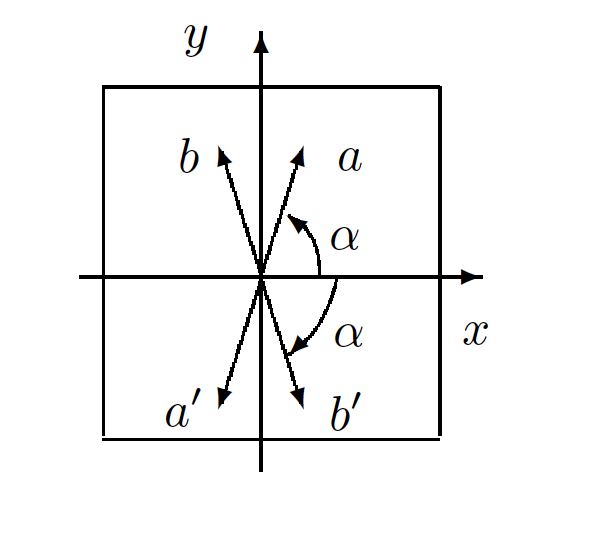
\includegraphics[width=\linewidth]{2.png}
	\caption{Поворот направления колебаний с помощью пластинки в $ \lambda / 2 $}
	\label{ris 2}
\end{wrapfigure}


Рассмотрим практически важные частные случаи.

 \begin{enumerate}
 		
 	\item Пластинка даёт сдвиг фаз $ 2\pi $ (пластинка в длину волны $ \lambda $). В результате сложения волн на выходе пластинки образует-
ся линейно поляризованная волна с тем же направлением колебаний, что и в падающей волне.

	\item Пластинка даёт сдвиг фаз $ \pi $ (пластинка в полдлины волны $ \lambda / 2 $). На выходе пластинки снова образуется линейно поляризованная волна. Направление $ bb' $ колебаний этой волны повёрнуто относительно направления $ aa' $ колебаний падающей волны (рис. 2). Как нетрудно сообразить, направление $ bb' $ является зеркальным отображением направления $ aa' $ относительно одного из главных направлений пластинки. Такую пластинку используют для поворота направления колебаний линейно поляризованного света.
	
	\item Пластинка создаёт между колебаниями сдвиг фаз $ \pi/2 $ (пластинка
в четверть длины волны). При сложении двух взаимно перпендикулярных колебаний, имеющих разность фаз $ \pi/2 $, образуется эллипс, главные оси которого совпадают с координатными осями $ x $ и $ y $. При равенстве амплитуд возникает круговая поляризация.
 	
 \end{enumerate}

Следует отметить, что, говоря о пластинках $ \lambda , \lambda/2, \lambda/4  $ и т. д., всегда подразумевают какую-либо вполне определённую монохроматическую
компоненту (например, пластинка $ \lambda/2 $ для зелёного света). Если на двоякопреломляющую пластинку падает не монохроматический свет, то на
выходе из неё для разных спектральных компонент эллипсы поляризации будут различными.

\subsection{Анализ эллиптически поляризованного света}

Анализ эллиптически поляризованного света сводится к нахождению главных осей
эллипса поляризации и к определению направления вращения электрического вектора.

Главные оси эллипса поляризации определяются с помощью анализатора по максимуму и минимуму интенсивности проходящего света.
Направление вращения электрического вектора может быть найдено
с помощью пластинки в четверть длины волны, для которой известно,
какая из главных волн, $ E_x $ или $ E_y $, имеет б\'{o}льшую скорость распространения (и соответственно меньшее значение показателя преломления).

Выберем для определённости координатные оси x и y на пластинке
так, чтобы $ nx < ny $. В этом случае главная волна $ E_x $ имеет большую
скорость распространения. Поместим такую пластинку на пути эллиптически поляризованного света и совместим главные направления пластинки $ \lambda/4 $ с главными осями эллипса поляризации. На выходе из этой
пластинки сдвиг фаз между $ E_x $ и $ E_y $ вместо $ \pi/2 $ станет равным ну-
лю или $ \pi $. Свет окажется линейно поляризованным. Из двух возможных значений сдвига фаз, 0 или $ \pi $, реализуется одно: то, которое соответствует имеющемуся в волне направлению вращения электрического вектора.

Рассмотрим, например, случай, когда электрический вектор в эллиптически поляризованной волне вращается против часовой стрелки,
если смотреть навстречу лучу. В этом случае, очевидно, в волне, падающей на пластинку в $ \lambda/4 $, колебание $ E_y $ отстаёт по фазе на $ \pi/2 $ от
колебания $ E_x $. При прохождении через пластинку разность фаз увеличивается до $ \pi $. Таким образом на выходе из пластинки возникают линейно поляризованные волны со сдвигом фаз $ \pi $. Сложение этих волн
даёт плоскополяризованную волну, электрический вектор которой рас-
полагается во втором и четвёртом квадрантах координатной системы
$ x, y $.

Рассуждая аналогичным образом, найдём, что при вращении электрического вектора по часовой стрелке направление колебаний в линейно поляризованной волне, выходящей из пластинки, располагается в первом и третьем квадрантах. Определяя направление колебаний на выходе из пластинки с помощью поляроида, можно, таким образом, определить характер эллиптической поляризации (вращение против или по часовой стрелке).

\subsection{Пластинка чувствительного оттенка}

\begin{wrapfigure}{l}{0.35\linewidth}
	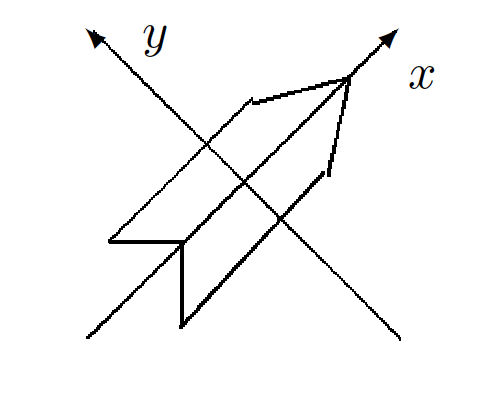
\includegraphics[width=\linewidth]{3.png}
	\caption{Пластинка
чувствительного
оттенка}
	\label{ris 3}
\end{wrapfigure}

Выше предполагалось известным, какому из двух главных направлений пластинки в четверть длины волны соответствует большая скорость распространения света.
Установить это можно различными способами, например с помощью
пластинки чувствительного оттенка (так называют пластинку в $ \lambda $
для зелёной спектральной компоненты, $ \lambda = 560 $ нм).

Пластинка имеет форму стрелы (рис. 3), вдоль оси которой расположено главное направление, соответствующее большей скорости распространения.

Если пластинка чувствительного оттенка помещена между скрещенными поляроидами и главные направления пластинки не параллельны
направлениям разрешённых колебаний поляроидов, то при освещении
белым светом пластинка кажется окрашенной в лилово-красный цвет.
Это объясняется тем, что зелёная компонента линейно поляризованного света при прохождении пластинки не меняет поляризации и задерживается вторым поляроидом. Для красной и фиолетовой компонент
пластинка создаёт сдвиг фаз, несколько отличный от $ 2\pi $. На выходе
из пластинки красная и фиолетовая компоненты оказываются поэтому
эллиптически поляризованными и частично проходят через второй поляроид. Таким образом, в известном смысле наблюдаемый в указанном
опыте цвет пластинки дополнителен к зелёному.

Если между скрещенными поляроидами поместить пластинку чувствительного оттенка
($ \lambda $) и пластинку в $ \lambda/4 $ так, чтобы их главные
направления совпадали, цвет пластинки изменится. Если у пластинки чувствительного оттенка и пластинки в $ \lambda/4  $совпадут главные направления, соответствующие большей скорости распространения, то разность хода между $ E_x $ и $ E_y $ для зелёного света составит уже $ 5\lambda/4 $. Это соответствует разности хода в $ \lambda $ для света с большей длиной волны, т. е. для "<более красного"> света. При освещении
этих пластинок (напомним, что они расположены между скрещенными поляроидами) белым светом теперь погасится не зелёная, а красная
часть спектра, и проходящий свет будет казаться зеленовато-голубым.
Если же главные направления, соответствующие большей скорости распространения, у пластинки чувствительного оттенка и у пластинки
в $ \lambda/4 $ окажутся перпендикулярными, то проходящий свет приобретёт
оранжево-желтую окраску (погасится фиолетово-голубая часть спектра).

Изменение цвета позволяет, таким образом, определить, какое из
главных направлений пластинки в $ \lambda/4 $ соответствует большей скорости
распространения.

\subsection{Интерференция поляризованных лучей}

\begin{wrapfigure}{r}{0.35\linewidth}
	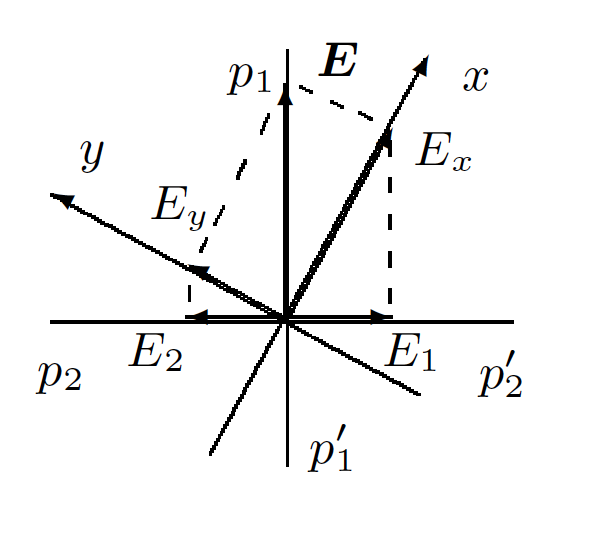
\includegraphics[width=\linewidth]{4.png}
	\caption{К объяснению интерференции
поляризованных лучей}
	\label{ris 4}
\end{wrapfigure}


Тонкие двоякопреломляющие пластинки, помещённые между поляроидами, кажутся окрашенными. Эта окраска может быть истолкована как результат интерференции поляризованных лучей. На рис. 4 представлена схема для
случая скрещенных поляроидов.

Здесь $ p1p'1 $ --- разрешённое направление колебаний поляризатора
(первого поляроида); $ x, y $ --- координатная система, связанная с главными направлениями двоякопреломляющей пластинки; $ p2p'2 $ --- разрешённое направление колебаний анализатора (второго поляроида). Волны
$ E_x  $ и $ E_y $ на выходе из пластинки когерентны, но не могут интерферировать, так как $ E_x \perp  E_y $. Волны $ E_1 $ и $ E_2 $ на выходе второго поляроида
также являются когерентными и к тому же поляризованы в одной плоскости. Эти волны интерферируют между собой. Результат интерференции определяется зависящим от длины волны сдвигом фаз между $ E_1 $
и $ E_2 $. В результате интерференции поляризованных лучей пластинка, освещаемая белым светом, кажется окрашенной.

Если поворачивать двоякопреломляющую пластинку, расположенную между
скрещенными поляроидами, то соотношение амплитуд волн $ E_1 $ и $ E_2 $ и разность фаз между ними не изменяются. Это означает, что цвет пластинки при её поворотах не меняется, а меняется только интенсивность света. За один оборот пластинки интенсивность четыре раза обращается в нуль --- это происходит при совпадении главных направлений
$ x $ и $ y $ с разрешёнными направлениями колебаний поляроидов.

Если же двоякопреломляющую пластинку оставить неподвижной, а
второй поляроид повернуть так, чтобы разрешённые направления $ p1p'1 $
и $ p2p'2 $ совпали, то волны $ E_1 $ и $ E_2 $ приобретают дополнительный фазовый сдвиг на $ \pi $ для всех спектральных компонент; при этом их амплитуды изменятся так, что цвет пластинки изменится на дополнительный. 


\section{Используемое оборудование}

\begin{enumerate}
    \item оптическая скамья с осветителем;
    \item зелёный светофильтр;
    \item два поляроида;
    \item чёрное зеркало;
    \item полированная эбонитовая пластинка;
    \item стопа стеклянных пластинок;
    \item слюдяные пластинки разной толщины;
    \item пластинки в 1/4 и 1/2 длины волны;
    \item пластинка в одну длину волны для зелёного света (пластинка чувствительного оттенка)
\end{enumerate}

\section{Результаты измерений и обработка данных}

%Параметры установки:
%\begin{description}
%\item{} $R_0 = 0,2~Ом$
%\item{} $R_и = 20~кОм$
%\item{} $C_и = 20~мкФ$
%\end{description}

\subsection{Определение разрешённых направлений поляроидов}

Разместим на оптической скамье осветитель, поляроид и чёрное зеркало (рис.~\ref{fig:polaroids}). Поворачивая поляроид вокруг направления луча, а чёрное зеркало вокруг вертикальной оси, добьёмся наименьшей яркости отражённого пятна. Такая конфигурация будет соответствовать горизонтальной поляризации света, прошедшего поляроид, так как при падении света на зеркало под углом Брюстера отражённый свет не будет содержать горизонтально поляризованную компоненту.

\begin{figure}[h!]
		\begin{minipage}[h!]{0.3\linewidth}
			\center{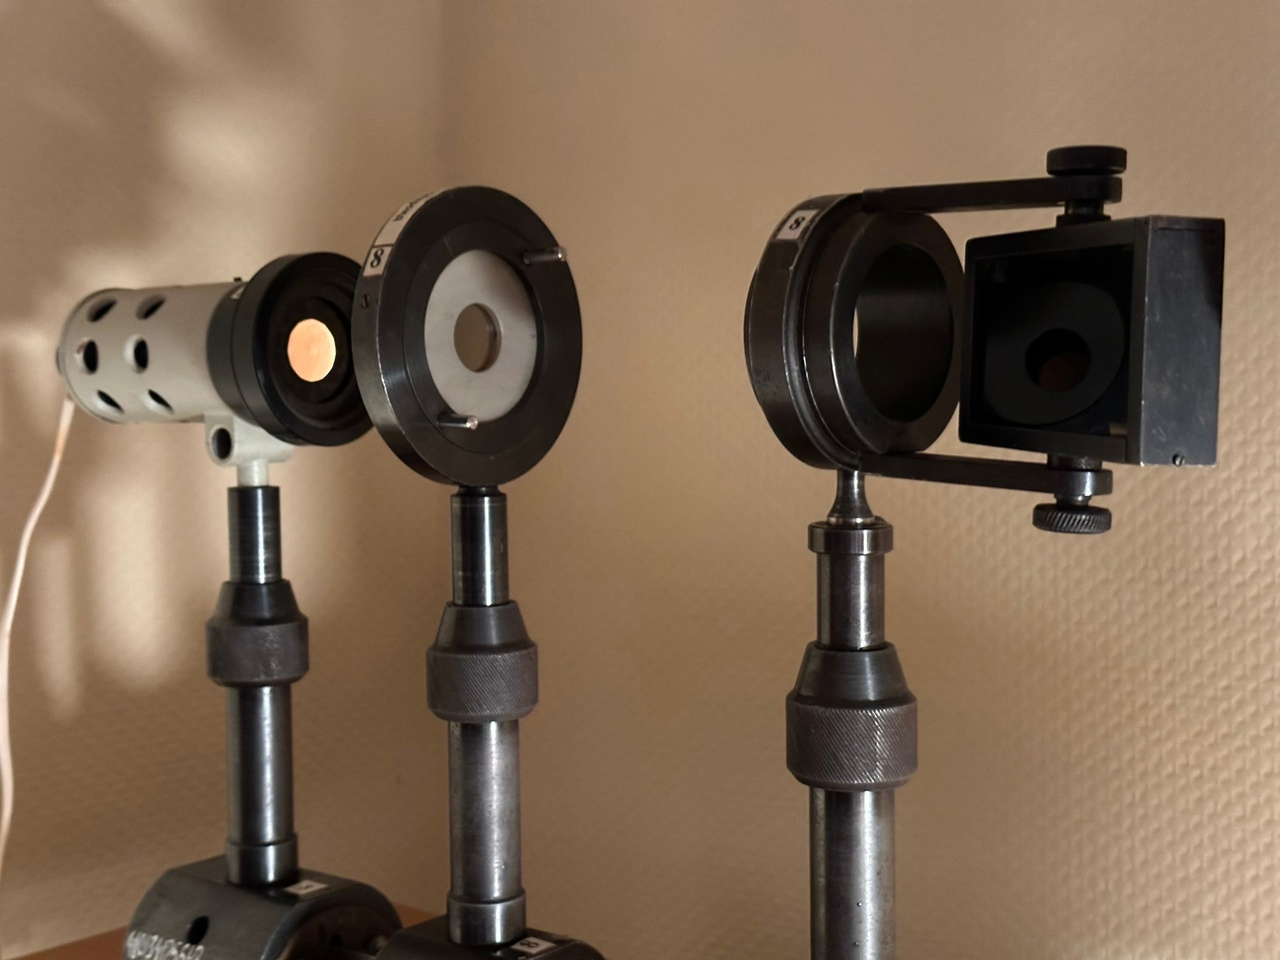
\includegraphics[width=1.2\linewidth]{polar1.jpg}}
		\end{minipage}
		\hfill
		\begin{minipage}[h!]{0.3\linewidth}
			\center{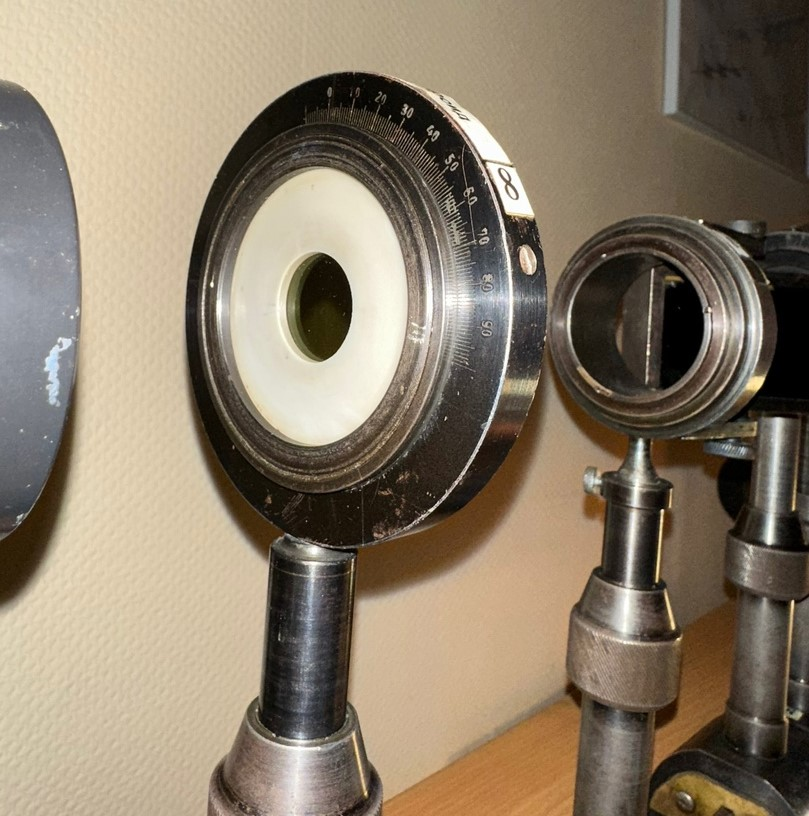
\includegraphics[width=1.2\linewidth]{polar2.jpg}}
		\end{minipage}
		\hfill
		\caption{Вид установки}
		\label{fig:polaroids}
\end{figure}

\newpage

\subsection{Определение показателя преломления эбонита}

Поставим на скамью вместо чёрного зеркала эбонитовую пластину (рис.~\ref{fig:ebonit}). По минимальной яркости отражённого света определим угол Брюстера для эбонита и рассчитаем по нему показатель преломления. $$\phi_B = 52^{\circ}\pm5^{\circ} \Rightarrow n_{э} = 1,07\div1,54.$$

\begin{figure}[h!]
        \begin{minipage}[h!]{0.3\linewidth}
			\center{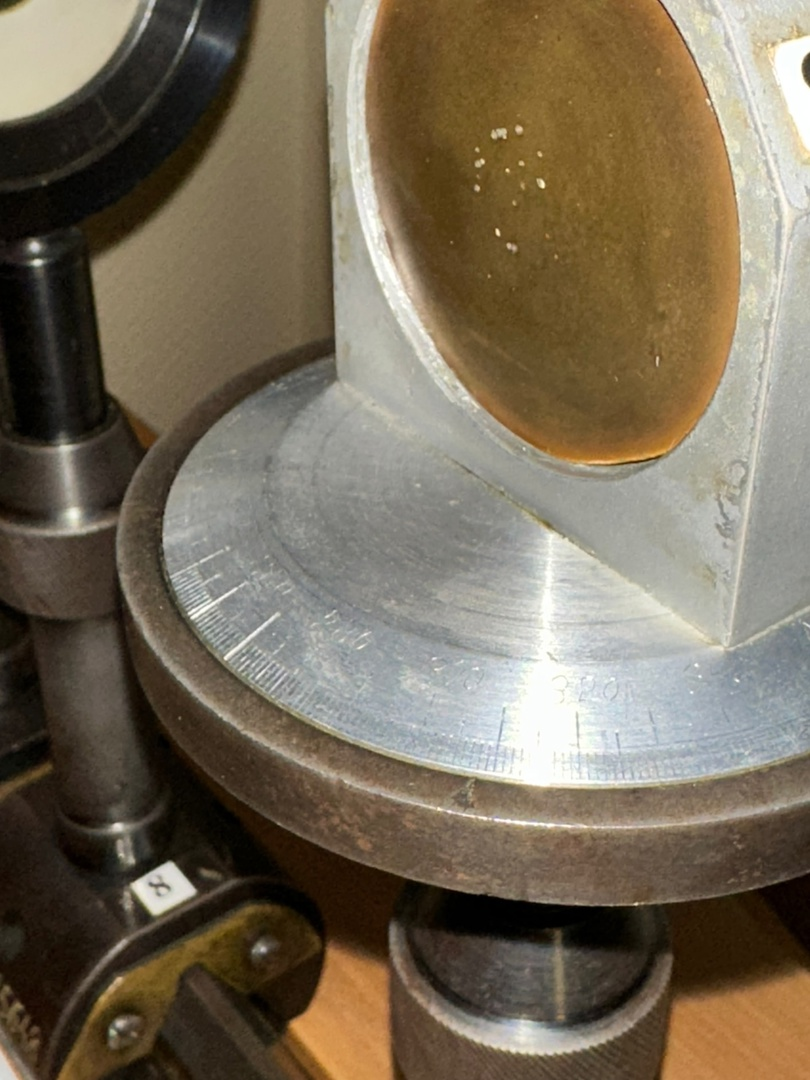
\includegraphics[width=1.2\linewidth]{ebonit1.jpg}}
		\end{minipage}
		\hfill
		\begin{minipage}[h!]{0.3\linewidth}
			\center{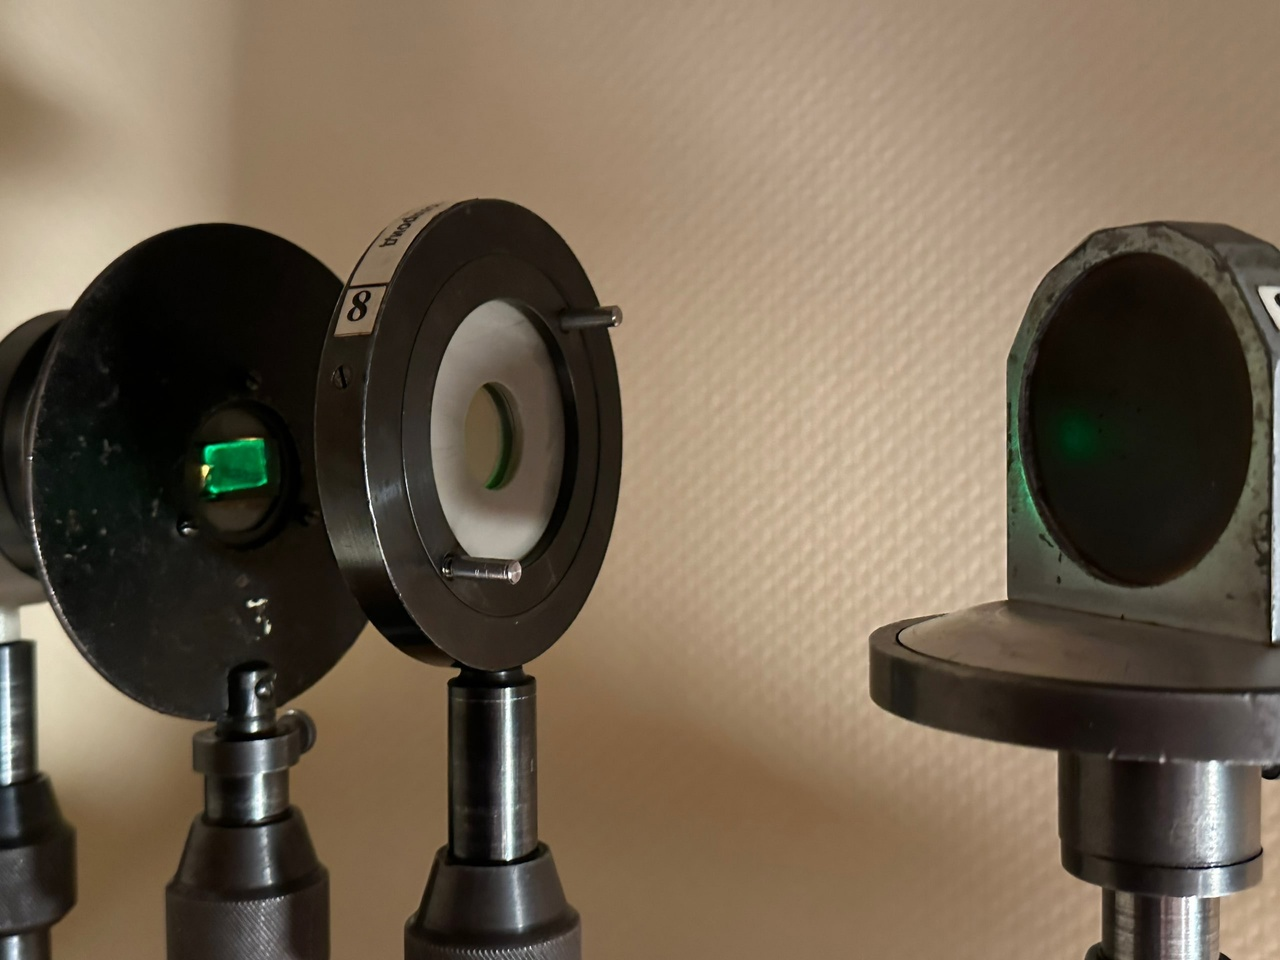
\includegraphics[width=1.2\linewidth]{ebonit2.jpg}}
		\end{minipage}
		\hfill
        \caption{Вид установки}
        \label{fig:ebonit}
\end{figure}

\newpage

\subsection{Исследование характера поляризации света в преломлённом и отражённом от стопы лучах}

Поставим вместо эбонитового зеркала стопу стеклянных пластинок под углом Брюстера (рис.~\ref{fig:stopa_ust}). Осветим стопу неполяризованным светом и, рассматривая через поляроиды отражённый от стопы и преломлённый лучи, определим в них ориентацию вектора $\mathbf{E}$.

\begin{figure}[h!]
\begin{center}
   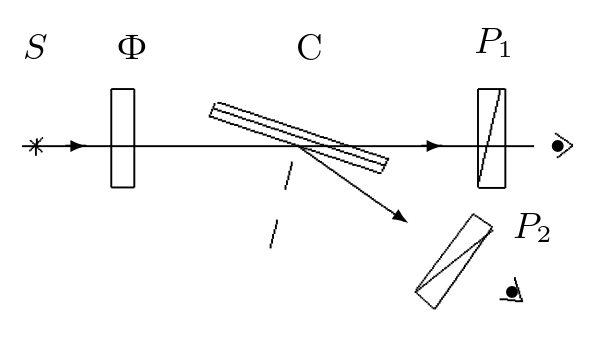
\includegraphics[width=0.8\linewidth]{stopa_ust.png}
\end{center}
\caption{Схема установки}
\label{fig:stopa_ust}
\end{figure}

\begin{figure}[h!]
        \begin{minipage}[h!]{0.3\linewidth}
			\center{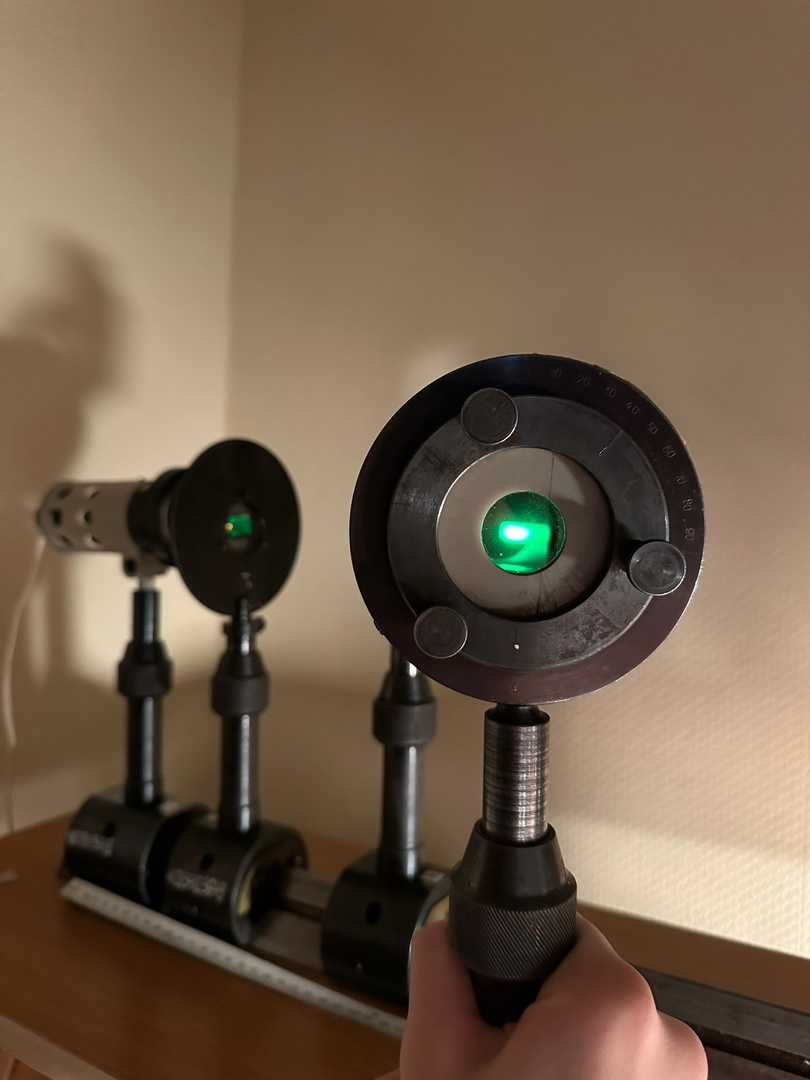
\includegraphics[width=1.2\linewidth]{stopa1.jpg} \\ в анализаторе с вертикальной поляризацией}
		\end{minipage}
		\hfill
		\begin{minipage}[h!]{0.3\linewidth}
			\center{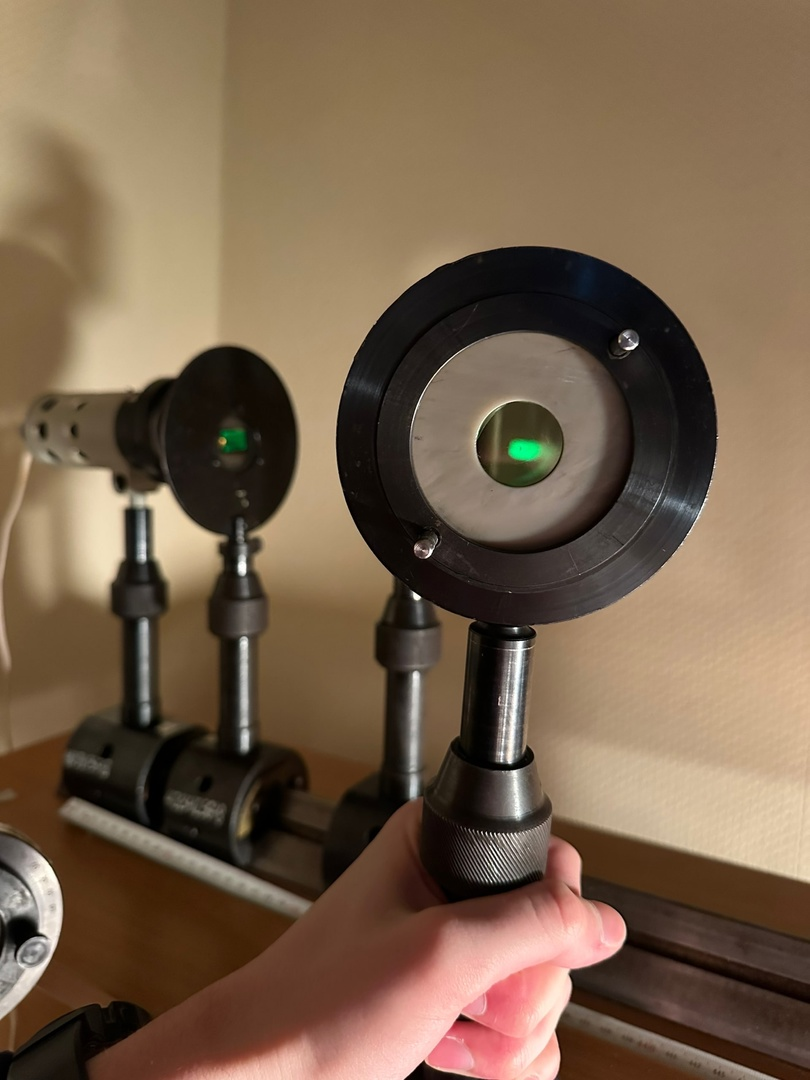
\includegraphics[width=1.2\linewidth]{stopa2.jpg} \\ в анализаторе с горизонтальной поляризацией}
		\end{minipage}
		\hfill
        \caption{Отражённый свет}
        \label{fig:stopa_reflektierte}
\end{figure}

\begin{figure}[h!]
        \begin{minipage}[h!]{0.3\linewidth}
			\center{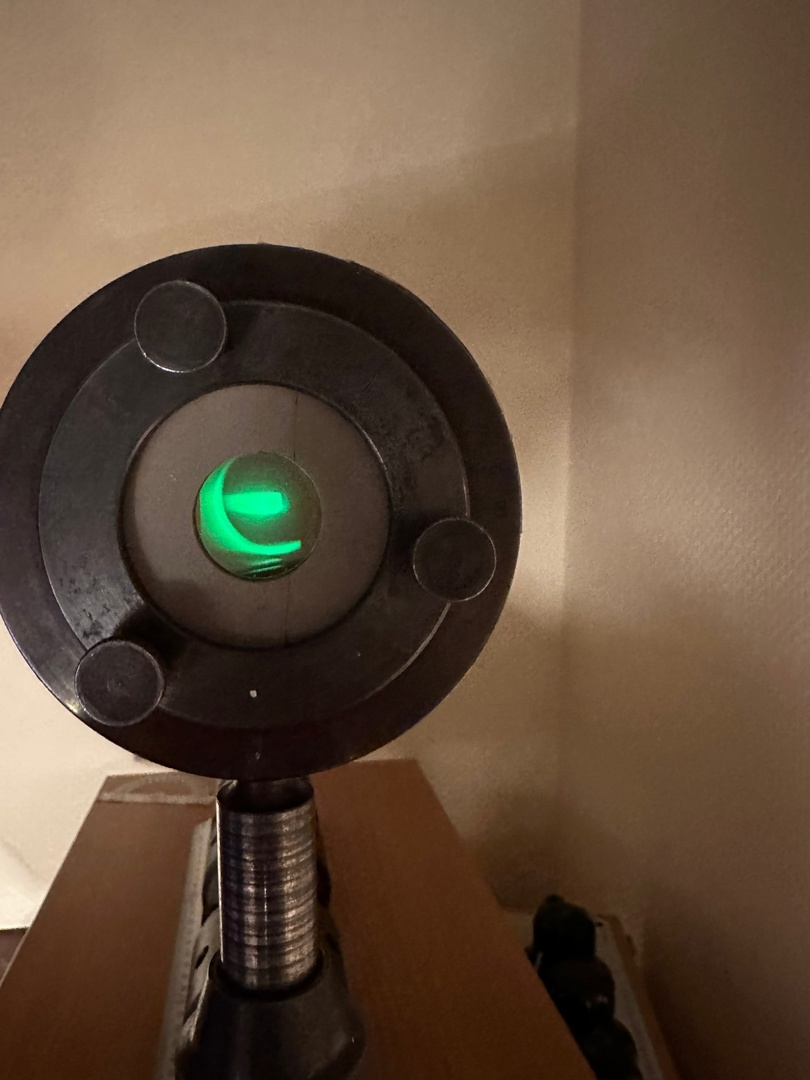
\includegraphics[width=1.2\linewidth]{stopa4.jpg} \\ в анализаторе с вертикальной поляризацией}
		\end{minipage}
		\hfill
		\begin{minipage}[h!]{0.3\linewidth}
			\center{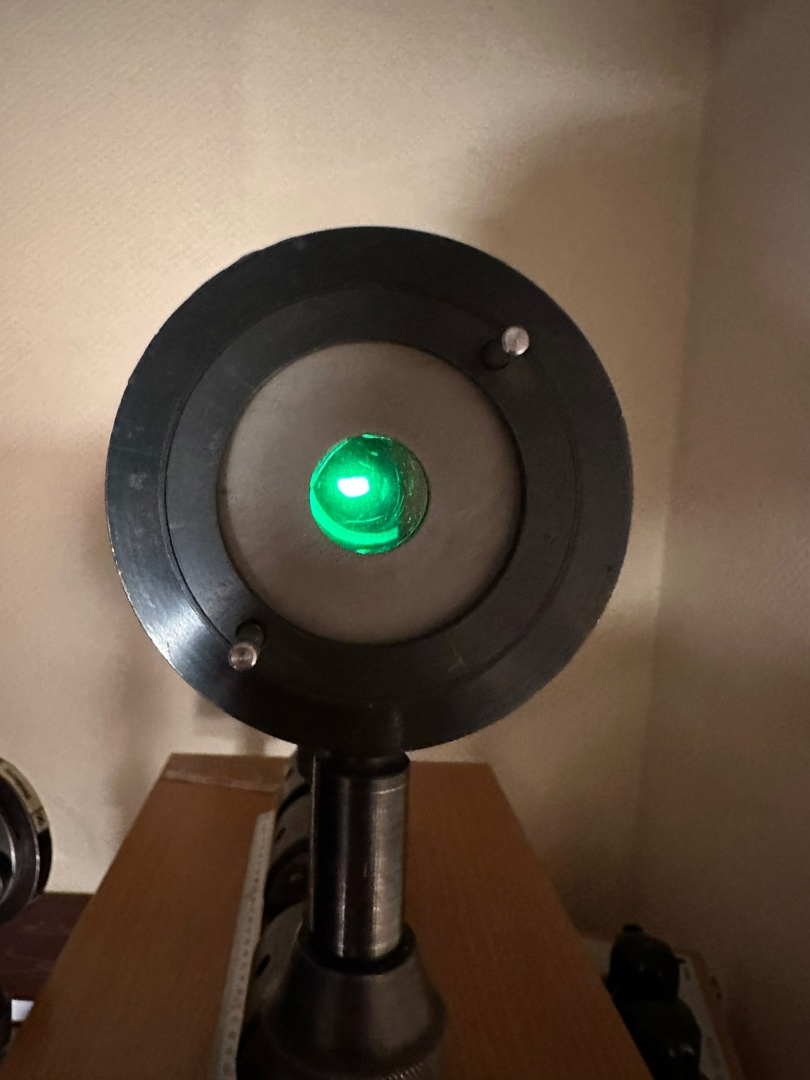
\includegraphics[width=1.2\linewidth]{stopa3.jpg} \\ в анализаторе с горизонтальной поляризацией}
		\end{minipage}
		\hfill
        \caption{Преломлённый свет}
        \label{fig:stopa_durchgehende}
\end{figure}

Отражённый свет (рис.~\ref{fig:stopa_reflektierte}) имеет б\'{о}льшую яркость, если смотреть на него через анализатор с вертикальной поляризацией, значит он имеет s-поляризацию (перпендикулярно плоскости падения). Аналогично, преломлённый свет (рис.~\ref{fig:stopa_durchgehende}) имеет p-поляризацию (в плоскости падения).

\newpage

\subsection{Определение главных направлений двоякопреломляющих пластин}

\begin{figure}[h!]
\begin{center}
   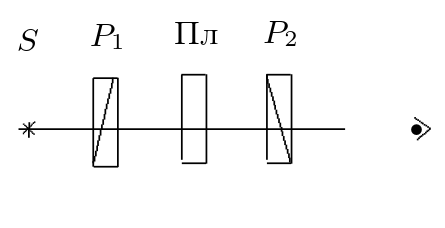
\includegraphics[width=0.5\linewidth]{plain_scheme.png}
\end{center}
\caption{Схема установки}
\label{fig:plain_scheme}
\end{figure}

Поставим кристаллическую пластинку между скрещенными поляроидами (рис.~\ref{fig:plain_scheme}). При вращении пластинки вокруг направления луча (рис.~\ref{fig:plain_ust}) интенсивность света будет минимальной при совпадении главных направлений пластинки с плоскостью поляризации, так как в этом случае свет перед пластинкой и после неё будет иметь горизонтальную поляризацию, и полностью погасится вторым поляроидом, имеющим вертикальную поляризацию (рис.~\ref{fig:plain_light}). Иначе получим на выходе эллиптическую поляризацию, и свет, пройдя через второй поляроид, будет иметь ненулевую интенсивность. Интенсивность будет максимальна, если угол между главными направлениями пластинки и плоскостью поляризации будет $45^{\circ}$ (круговая поляризация).

\begin{figure}[h!]
\begin{center}
   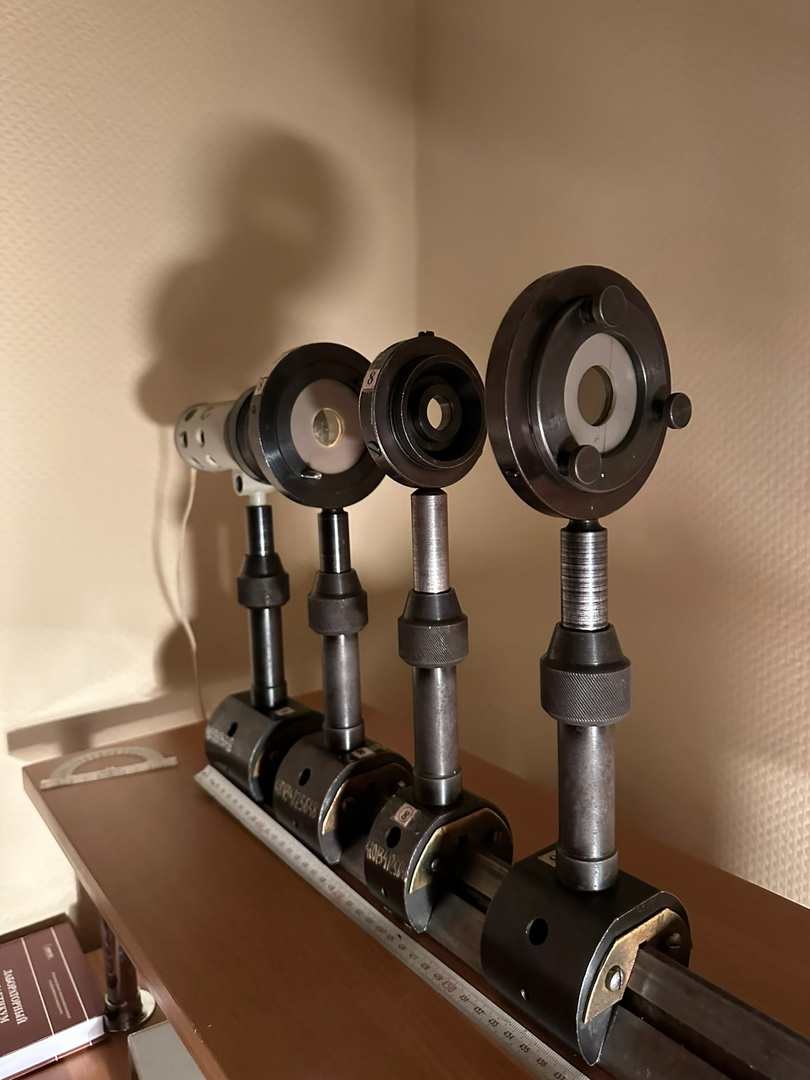
\includegraphics[width=0.4\linewidth]{plain_ust.jpg}
\end{center}
\caption{Вид установки}
\label{fig:plain_ust}
\end{figure}

\begin{figure}[h!]
        \begin{minipage}[h!]{0.3\linewidth}
			\center{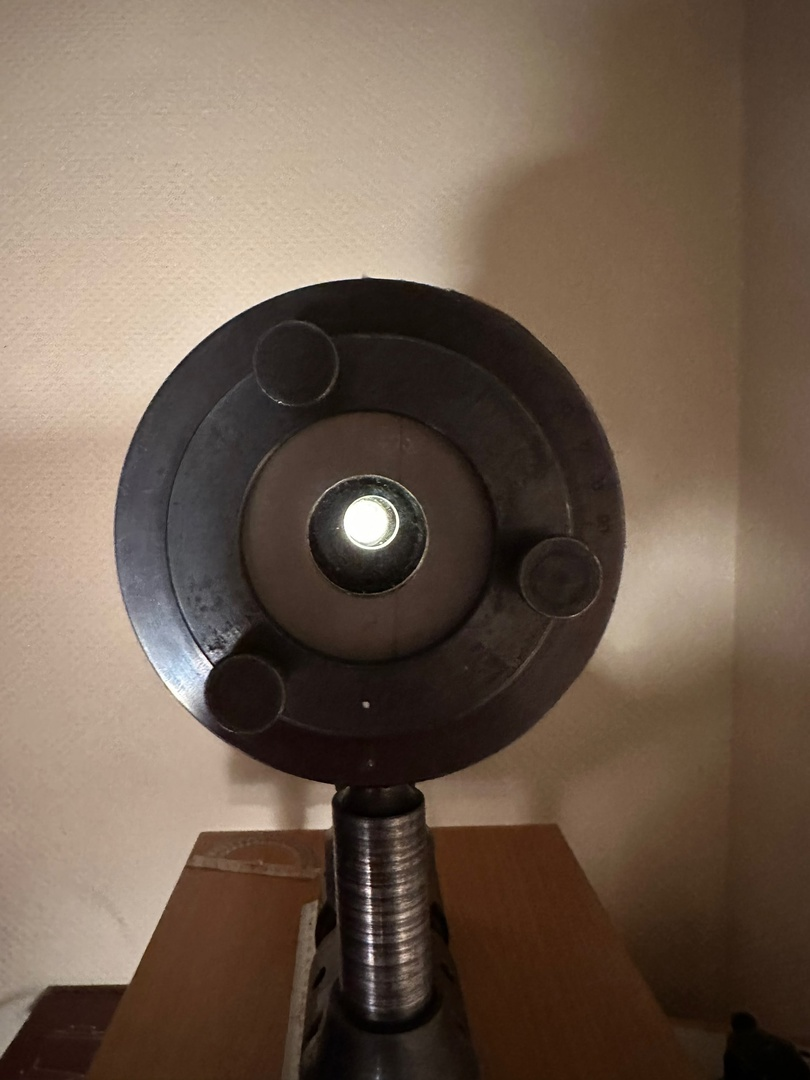
\includegraphics[width=1.2\linewidth]{plain_max.jpg} \\ максимальная интенсивность}
		\end{minipage}
		\hfill
		\begin{minipage}[h!]{0.3\linewidth}
			\center{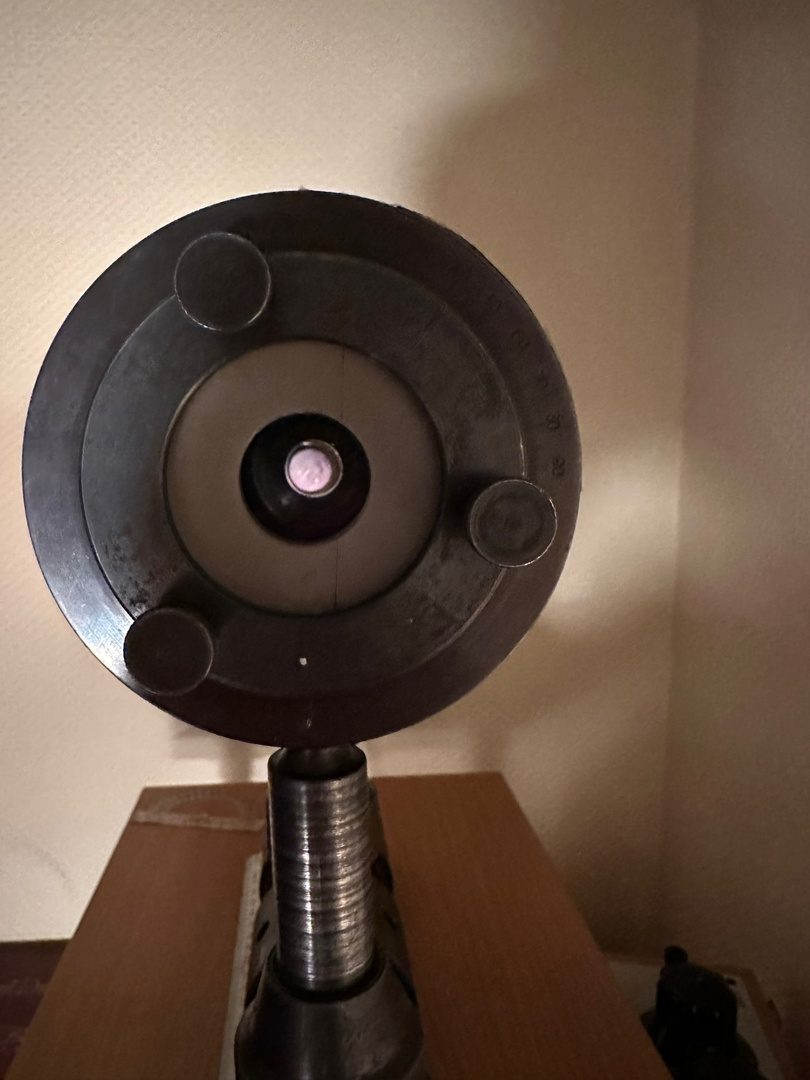
\includegraphics[width=1.2\linewidth]{plain_min.jpg} \\ минимальная интенсивность}
		\end{minipage}
		\hfill
        \caption{Прохождение света через двоякопреломляющую пластину}
        \label{fig:plain_light}
\end{figure}

\newpage

\subsection{Выделение пластин $\lambda/2$ и $\lambda/4$}

Добавим к схеме (рис.~\ref{fig:plain_scheme}) зелёный фильтр. Установим разрешённое направление первого поляроида горизонтально, а главные направления исследуемой пластинки --- под углом $45^{\circ}$ к горизонтали. Свет, прошедший через пластинку $\lambda/2$ будет иметь линейную поляризацию, и минимум интенсивности будет наблюдаться два раза за оборот второго поляроида. В случае пластинки $\lambda/4$ свет на выходе будет иметь эллиптическую поляризацию и существенные изменения интенсивности наблюдаться не будут.

\subsection{Определение <<быстрой>> и <<медленной>> оси в пластинке $\lambda/4$}

Поставим между скрещенными поляроидами пластинку чувствительного оттенка (рис.~\ref{fig:axes_scheme}), имеющую вид стрелки. Данная пластинка не будет менять поляризацию зелёного света. Если убрать зелёный фильтр, стрелка будет иметь пурпурный цвет (рис.~\ref{fig:axes_sensitive}), так как сдвиг фаз $2\pi$ для зелёного соответствует сдвигу фаз несколько отличному от $2\pi$ для других длин волн, т. е. волны других цветов буду иметь на выходе эллиптическую поляризацию, и пройдут через анализатор.

\begin{figure}[h!]
\begin{center}
   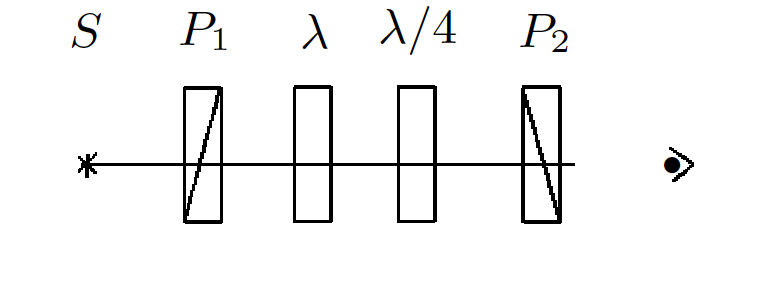
\includegraphics[width=0.7\linewidth]{axes_scheme.png}
\end{center}
\caption{Схема установки}
\label{fig:axes_scheme}
\end{figure}

\begin{figure}[h!]
\begin{center}
   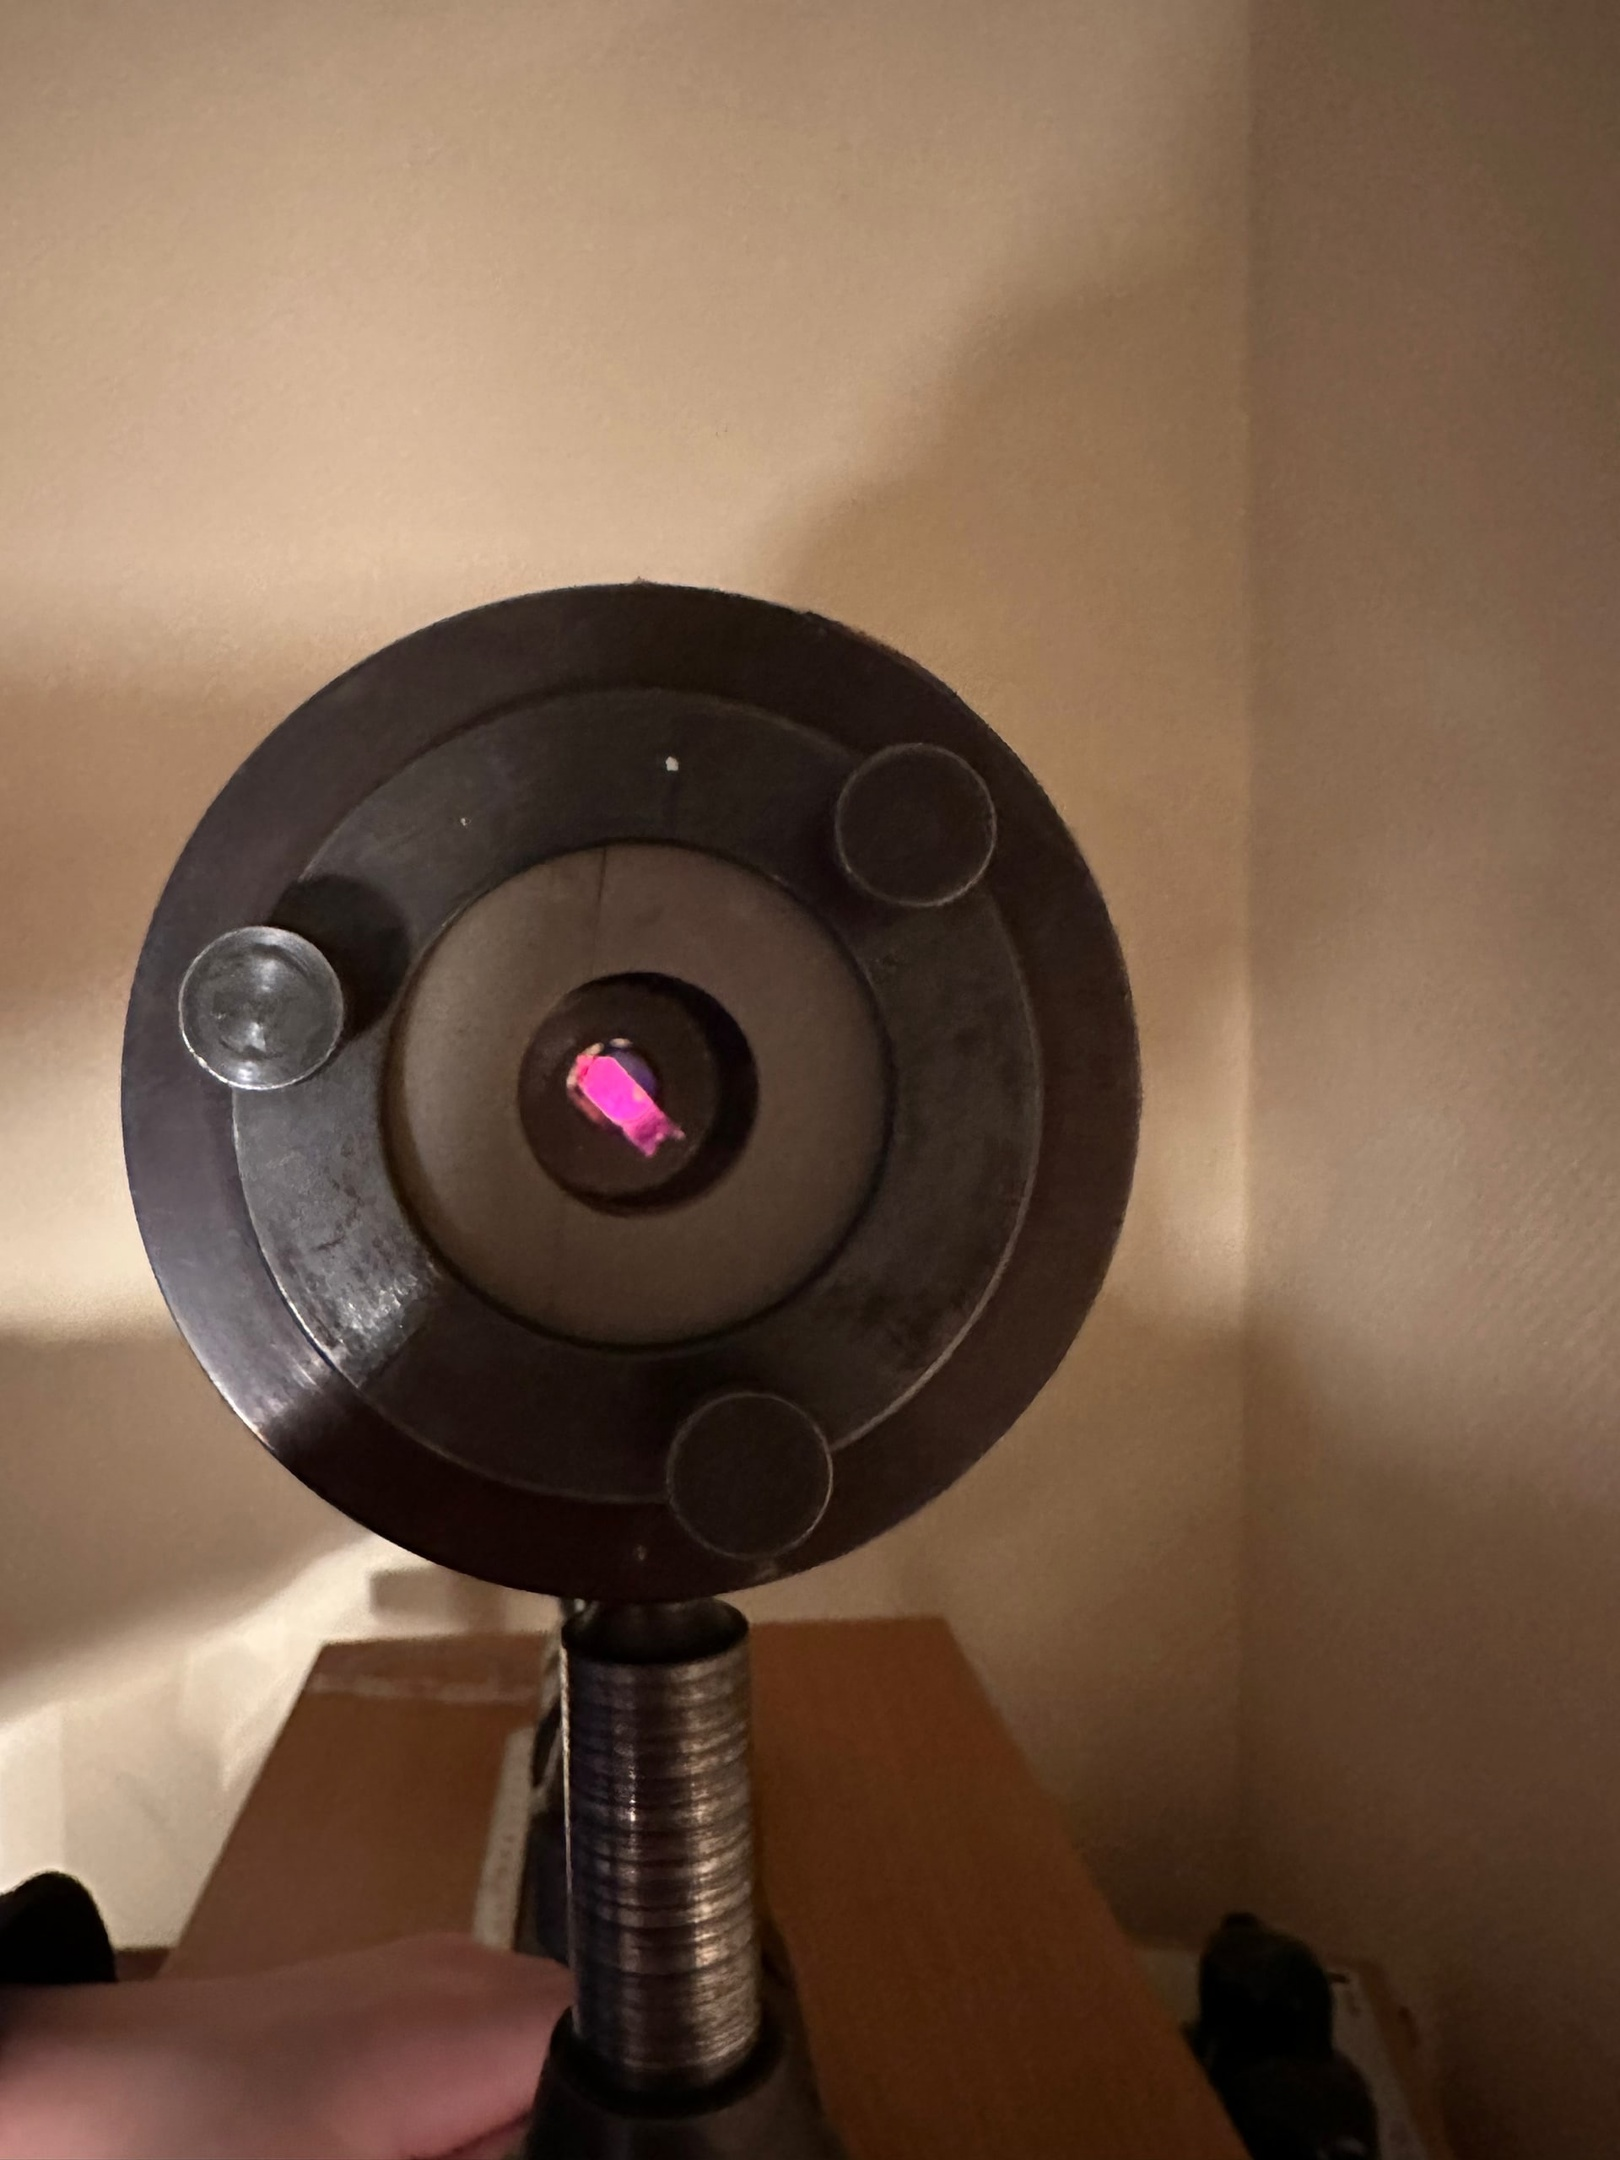
\includegraphics[width=0.5\linewidth]{axes_sensitive.jpg}
\end{center}
\caption{Пластинка чувствительного оттенка}
\label{fig:axes_sensitive}
\end{figure}

Добавим к схеме пластинку $\lambda/4$, главные направления которой совпадают с главными направлениями пластинки $\lambda$ и ориентированы под углом $45^{\circ}$ к разрешёнными направлениям скрещенных поляроидов. При повороте рейтера со стрелкой на $180^{\circ}$ вокруг вертикальной оси цвет стрелки меняется от зелёно-голубого до оранжево-жёлтого. Если главные направления пластин совпадают, то разность хода для зелёного цвета составляет $5\lambda/4$. Это значит, что волны ближе к красному цвету будут иметь разность хода $\lambda$ и не пройдут через анализатор, т. е. на выходе получится зелёно-голубой свет. В противном случае свет на выходе будет ближе к красному.

\newpage

\subsection{Интерференция поляризованных лучей}

Между скрещенными поляроидами расположим мозаичную слюдяную пластинку. Она собрана из 4-х узких плосок слюды, лежащих по сторонам квадрата (две полоски $\lambda/4$ и по одной $\lambda/2$ и $3\lambda/4$). В центральном квадратике слюды нет. Главные направления всех пластинок ориентированы параллельно сторонам квадрата. При вращении пластинки интенсивность света в каждом квадратике меняется 4 раза за оборот (рис.~\ref{fig:mosaic}), так как 4 раза за оборот оси пластинок совпадают с плоскостями поляроидов. При вращении поляроида квадратики будут менять цвет 4 раза за оборот.

\begin{figure}[h!]
\begin{center}
   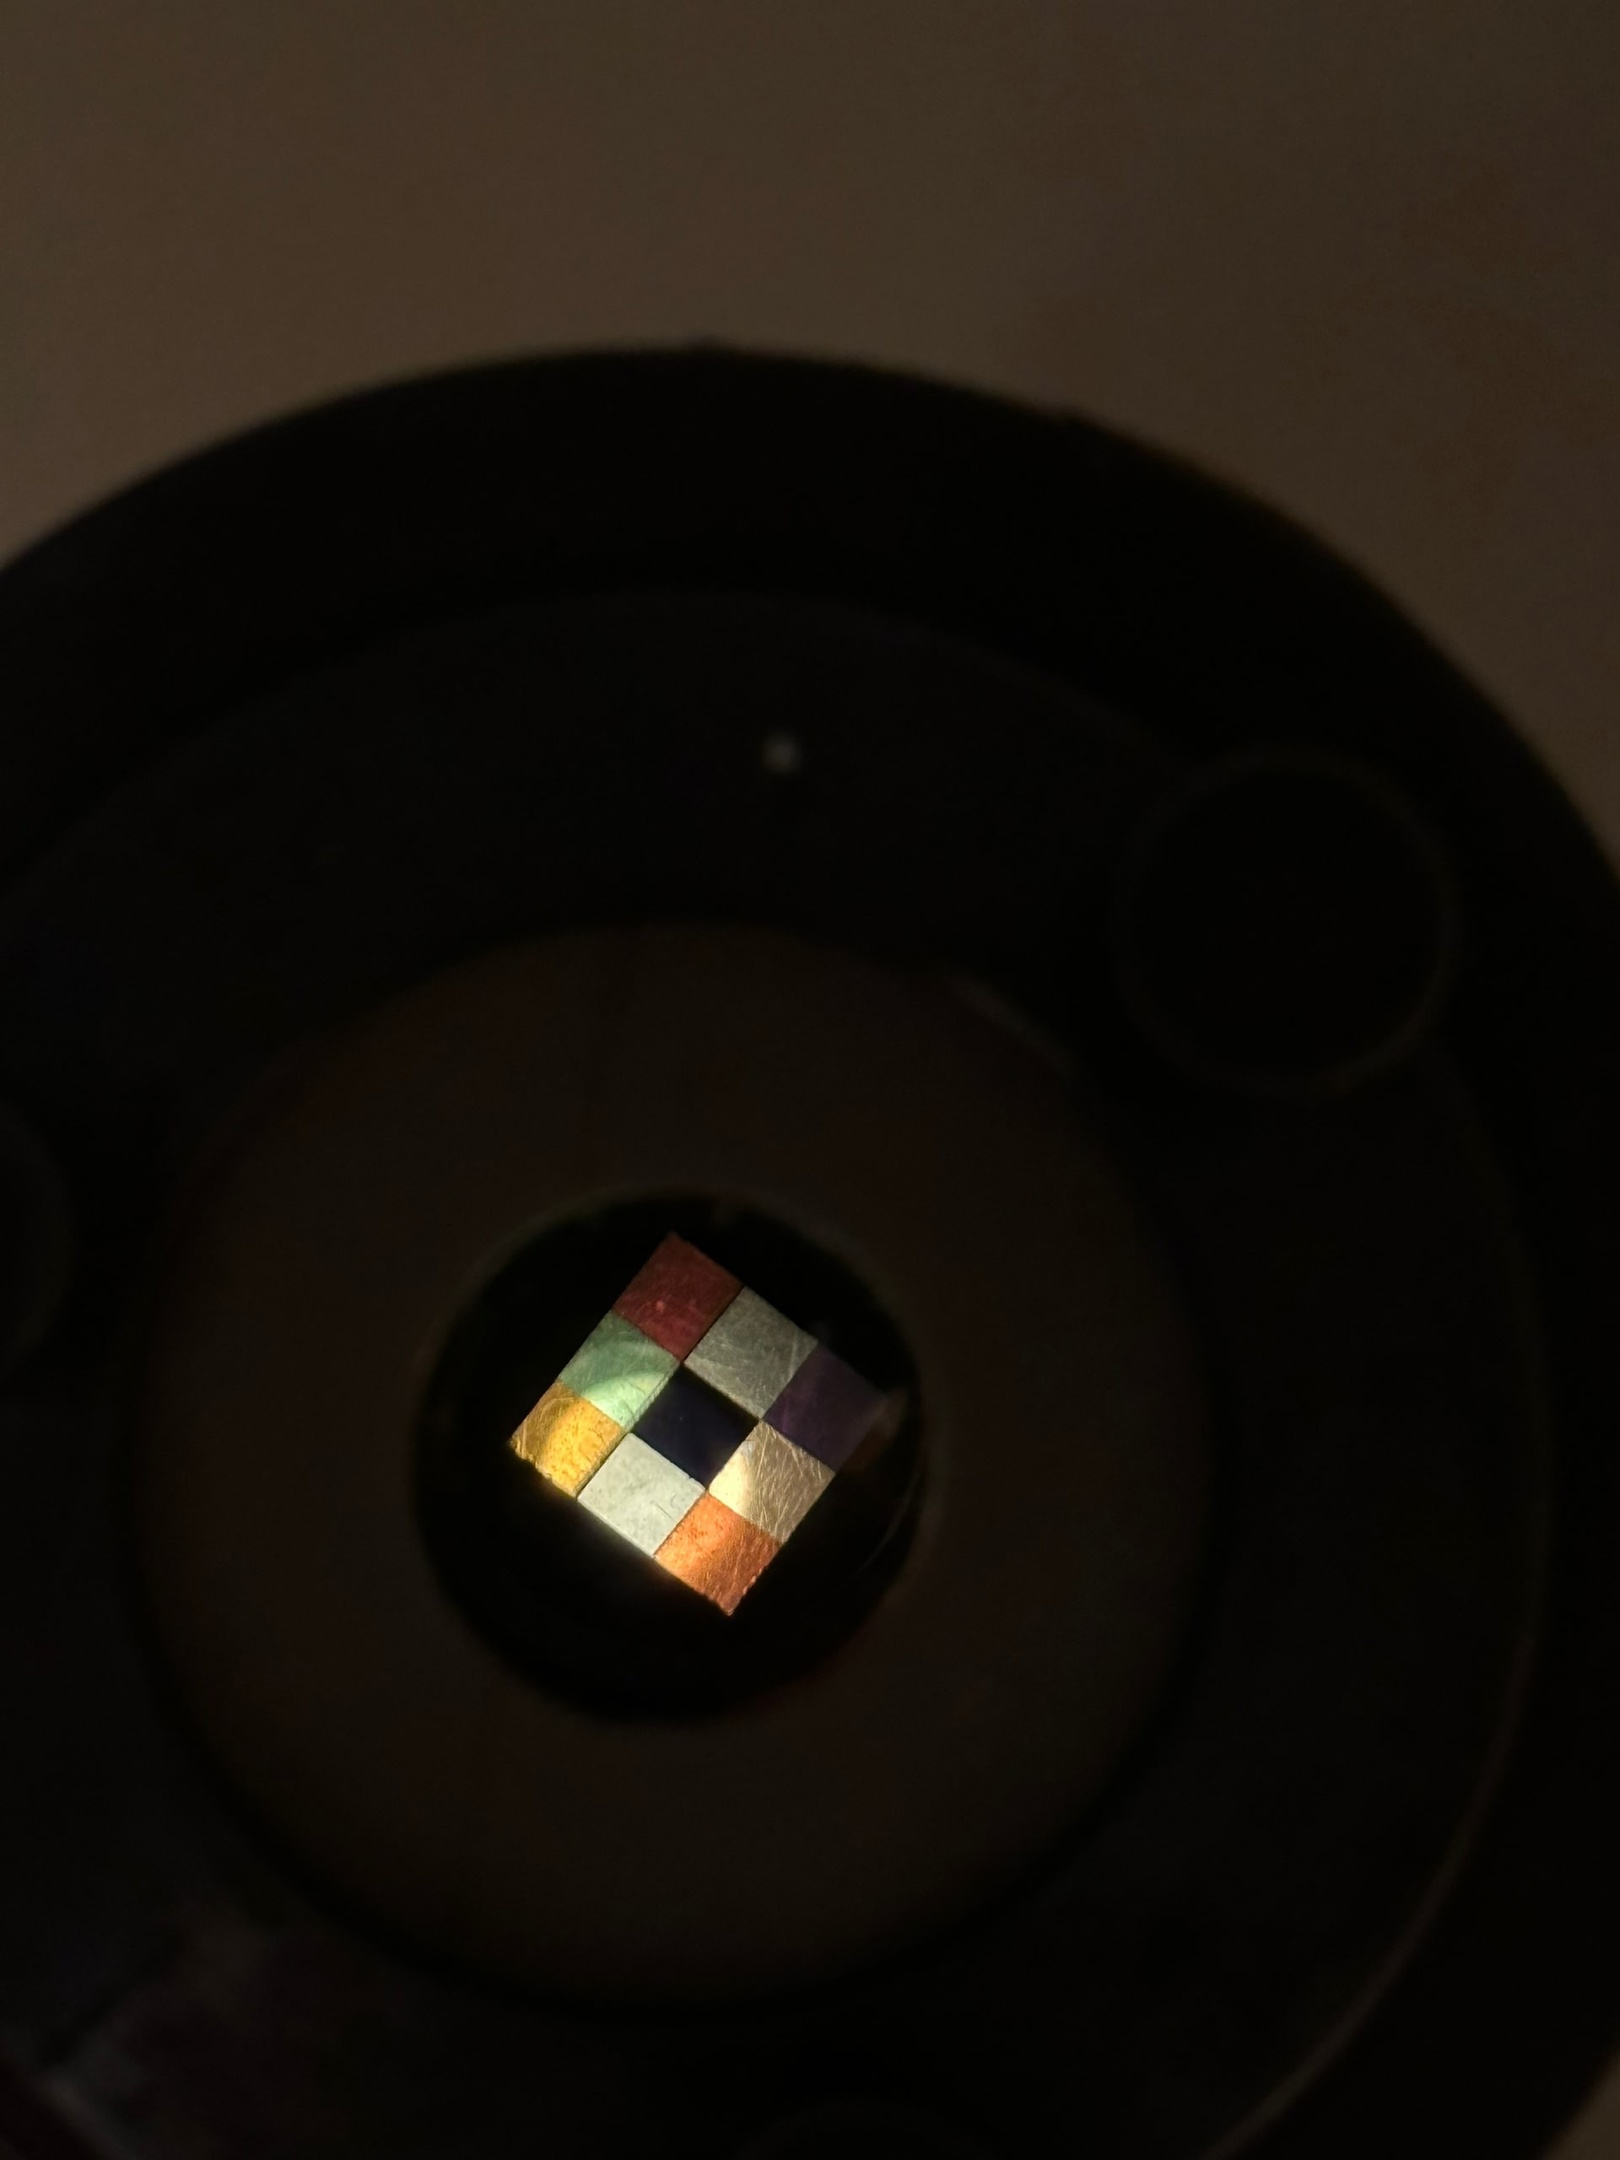
\includegraphics[width=0.5\linewidth]{mosaic.jpg}
\end{center}
\caption{Мозаичная пластинку между скрещенными поляроидами}
\label{fig:mosaic}
\end{figure}

\newpage

\subsection{Определение вращения светового вектора в эллиптически поляризованной волне}

На рис.~\ref{fig:rotation} показано направление вектора $\mathbf{E}$ на входе в пластинку и его эллиптическая поляризация на выходе из неё, а также зависимость от времени проекций светового вектора на координатные оси. В данном случае свет на выходе имеет левую поляризацию.

\begin{figure}[h!]
\begin{center}
   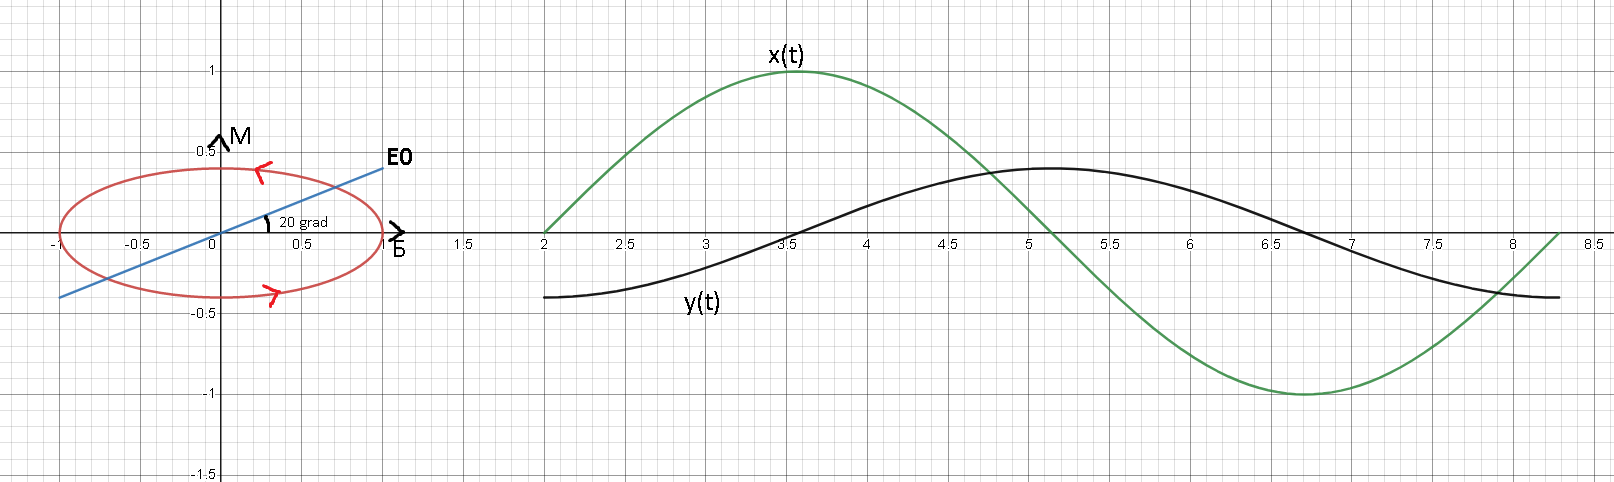
\includegraphics[width=1.0\linewidth]{rotation.png}
\end{center}
\caption{Изменение поляризации света при переходе через пластинку}
\label{fig:rotation}
\end{figure}

\section{Обсуждение результатов и выводы}

В данной работе были получены следующие результаты:
\begin{itemize}
\item Определены разрешённые направления поляроидов;
\item Был определен показатель преломления эбонита по измерению угла Брюстера:
\begin{equation*}
    \boxed{n = \tg{52^{\circ}\pm5^{\circ}} = 1,3\pm0,3}
\end{equation*}
Полученный результат в пределах погрешности согласуется с табличным $n = 1,6$;
\item Определена поляризация лучей, отражённых и преломлённых стопой стеклянных пластин. Отражённые лучи поляризованы вертикально, а преломлённые --- горизонтально;
\item Для двоякопреломляющих пластин определены главные направления. Минимумы и
максимумы интенсивности чередуются через четверть оборота, главные оси пластин совпадают с разрешенными направлениями поляроидов при максимальной интенсивности;
\item Были выделены пластинки с разностью хода $\lambda/2$ и $\lambda/4$;
\item «Быстрая» ось пластинки $\lambda/4$ имеет направление $150^{\circ}$ по шкале рейтера, а <<медленная>> --- $240^{\circ}$;
\item При изучении интерференции поляризованных лучей было получено, что при вращении пластинки в отдельном квадратике изменяется интенсивность, а при вращении анализатора --- изменяется цвет;
\end{itemize}

\end{document}
